% !TEX encoding = UTF-8 Unicode
\documentclass[12pt]{article}
\usepackage{kotex}
\usepackage{graphicx}
\DeclareGraphicsExtensions{.pdf,.png,.jpg}
\pagestyle{plain}
\setcounter{secnumdepth}{2}

\topmargin=0cm
\oddsidemargin=0cm
\textheight=22.0cm
\textwidth=16cm
\parindent=0cm
\parskip=0.15cm
\topskip=0truecm
\raggedbottom
\abovedisplayskip=3mm
\belowdisplayskip=3mm
\abovedisplayshortskip=0mm
\belowdisplayshortskip=2mm
\normalbaselineskip=12pt
\normalbaselines

\begin{document}

\vspace*{0.5in}
\centerline{\bf\Huge Requirements Document}
\thispagestyle{empty}
\vspace*{0.5in}
\centerline{\bf\Large Team 2}

\vspace*{0.5in}
\centerline{\bf\Large 21 October 2016}

\vspace*{1.5in}
\begin{table}[b]
\caption{Team Member}
\begin{center}
\begin{tabular}{| c | c |}
\hline
ID Number & Name \\
\hline\hline
122290 & 이재환 \\
\hline
122308 & 김태형 \\
\hline
13012672 & 김남우 \\
\hline
13012673 & 이찬형 \\
\hline
\end{tabular}
\end{center}
\end{table}

\newpage
\thispagestyle{empty}
\begin{table}[hbpt]
\caption{Revision Control}
\begin{center}
\begin{tabular}{| c | c | c |}
\hline
Version & Date & Description \\
\hline\hline
1.0 & `16. 10. 21. & Start a project of developing Sudoku system \\
\hline
 & & \\
\hline

\end{tabular}
\end{center}
\end{table}

\clearpage
\thispagestyle{empty}
\tableofcontents
\listoffigures
\listoftables
\newpage

\clearpage

\section{System}
Sudoku is a puzzle game designed for a single player.
Grids are stacked nine high and nine wide, making 81 grids total. 
The puzzle comes with some of the girds already filled in, and the player guess the values of empty grids with some sudoku rules.

\subsection{Purpose}
This document is to define requirements for Sudoku system.
The intended audience of this document is describes in table below.
\begin{table}[h]
\begin{center}
\begin{tabular}{| l | l |}
\hline
Group of the readers & Reasons for reading \\
\hline\hline
User and customers & To give feedback about the requirements \\
\hline
System developers & To understand what functions and properties the system must contain \\
\hline
Testers & To test the system against the requirements \\
\hline
Project team & To follow-up the status of the project against the requirements \\
\hline
\end{tabular}
\end{center}
\caption{Intended audience of this document}
\end{table}
%\subsection{Context}

%\subsection{Business Goals}
\section{Domain Model}
Before specific requirements were identified, a domain analysis (see following figure and description) was conducted to identify essential concepts. \\
\begin{figure}[h]
\begin{center}
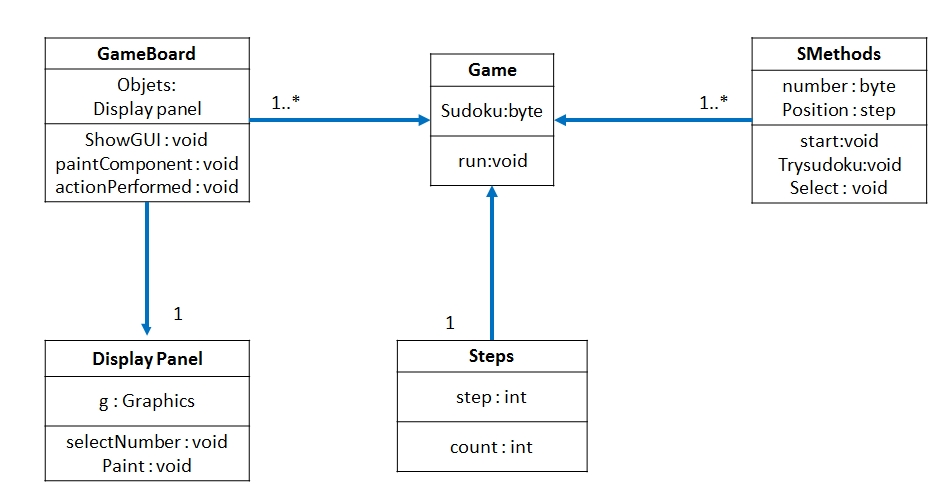
\includegraphics[scale=0.43]{domain_model.jpg}
%insert diagram here
\label{fig:domain-model}
\end{center}
\caption{Domain Model}
\end{figure}

\begin{table}[h]
\begin{center}
\begin{tabular}{| l | l |}
\hline
Concept name & Description \\
\hline\hline
GameBoard & 'GameBoard' is a puzzle board displayed on the screen \\
\hline
Game & 'Game' is a set of sudoku game \\
\hline
SMethods & 'SMethods' is sudoku methods generate puzzle, and check the result  \\
\hline
Display panel &  'Display panel' display all the components to be displayed on the game screen \\
\hline
Steps & 'Steps' indicate step of how many times user input values in the grids. \\
\hline
\end{tabular}
\end{center}
\caption{Domain concepts}
\end{table}

\section{Actors}
Any user who know how to play a sudoku game can be an actor of this program.
\section{Use Cases}

\subsection{Overview}
We proposed to develop sudoku puzzle which is satisfied three conditions.
The first version that we develop in here is minimal version.
This version produce basic function and user interface of sudoku puzzle.
The user can input numbers of 1 to 9 into grids of sudoku puzzle.
After all the grids are filled, the user can check the result of the game.\\
\begin{figure}[h]
\begin{center}
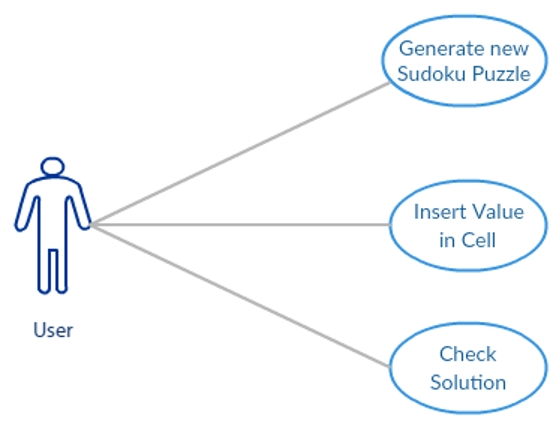
\includegraphics[scale=0.5]{use_case_diagram.jpg}
%insert diagram here
\caption{Use Case Diagram}
\label{fig:use-case-diagram}
\end{center}
\end{figure}

\subsubsection{Use Case 1} \label{uc:1}
\noindent
{\bf Name}\\
Generating a new puzzle\\

\noindent
{\bf Summary}\\
When the user open this program and click the 'Start' button, the sudoku generator will make a set of game. Each game has 81(9*9) grids.\\
%A short summary/description/story.

\noindent
{\bf Actors}\\
Any user. \\

\noindent
{\bf Precondition}\\
A executable file of this game should be provided to the user.\\

\noindent
{\bf Main Scenario}\\
\vspace*{-0.2in}
\begin{enumerate}
\item 
The user double click the executable file of sudoku game.
\item
The system provide a 'Start Your Sudoku' button on the game screen.
\item
The user click the button.
\item
The new set of game is generated on the game screen.
\end{enumerate}

\noindent
{\bf Exceptions}\\
N/A \\

\noindent
{\bf Postcondition}\\
The user can input a number into grids.\\

\noindent
{\bf Priority}\\
Must \\

\noindent
%{\bf Traces to Test Cases}\\
%Add when test cases done.

\subsubsection{Use Case 2} \label{uc:2}

\noindent
{\bf Name}\\
Inserting a value into a grid\\

\noindent
{\bf Summary}\\
The user can input a number(only 1 to 9) into an empty grid.\\
%A short summary/description/story.

\noindent
{\bf Actors}\\
Any user. \\

\noindent
{\bf Precondition}\\
The user must be executing the sudoku program.\\

\noindent
{\bf Main Scenario}\\
\vspace*{-0.2in}
\begin{enumerate}
\item 
The system has many empty(not selected) grid that waiting for number.
\item
A grid have small nine numbers(1 to 9) on it and user can click on of them.
\item
The user click a number in an empty grid.
\item
The grid will have just one bigger number user selected.
\end{enumerate}

\noindent
{\bf Exceptions}\\
N/A\\

\noindent
{\bf Postcondition}\\
The user can check after all the grids are filled whether all the values are located correctly.\\

\noindent
{\bf Priority}\\
Must \\

\noindent
%{\bf Traces to Test Cases}\\
%Add when test cases done.

\subsubsection{Use Case 3} \label{uc:3}

\noindent
{\bf Name}\\
Check success or failure\\

\noindent
{\bf Summary}\\
The user can check the success or failure of the game, after all the grids have their value.\\
%A short summary/description/story.

\noindent
{\bf Actors}\\
Any user. \\

\noindent
{\bf Precondition}\\
The user should fill all the grids with valid number(1 to 9).\\

\noindent
{\bf Main Scenario}\\
\vspace*{-0.2in}
\begin{enumerate}
\item 
The user fill all the empty grid with a valid number(1 to 9).
\item
The system give a message when all grids are full, success or failure.
\end{enumerate}

\noindent
{\bf Exceptions}\\
If all the grids were not filled, the system can't check the result.\\

\noindent
{\bf Postcondition}\\
The user can get a message about success or failure. \\

\noindent
{\bf Priority}\\
Must \\

\noindent
%{\bf Traces to Test Cases}\\
%Add when test cases done.

\section{Non-Functional Constraints}
\subsection{Product requirement}
\subsubsection{Usability requirement}
\begin{itemize}
%\item Sudoku game support the three levels that include easy, normal and hard and User can select the sudoku game and play the game by input the number into squares.
\item 
\item User can note numbers in each squares.
\item When squares are full, the system shall inform success or fail.
\end{itemize}
\subsection{Organizational requirement}
\subsubsection{Implement requirement}
\begin{itemize}
\item All code for sudoku game must be written by using JAVA language.
\item This project should follow incremental development method.
\end{itemize}

%\section{Data Dictionary}

\section{References}
N/A
\appendix % Annex ..

%\section{Description of File Format: Tasks}

%Describe input file format.

%\section{Description of File Format: Persons}

%Describe output file format.

\end{document}
